\documentclass[tikz,border=8pt]{standalone}
% Shared look for every TikZ diagram. Load with % Shared look for every TikZ diagram. Load with % Shared look for every TikZ diagram. Load with \input{../../tools/tikz-style.tex}
\usepackage[T1]{fontenc}
\usepackage{lmodern}
\renewcommand{\sfdefault}{lmr}  % diagrams use the same serif as the text
\usetikzlibrary{arrows.meta, positioning, shapes.geometric, calc, fit, backgrounds}
\definecolor{cblue}{HTML}{4C78A8}
\definecolor{corange}{HTML}{F58518}
\definecolor{cgreen}{HTML}{54A24B}
\definecolor{cred}{HTML}{E45756}
\definecolor{cpurple}{HTML}{B279A2}
\definecolor{cgrey}{HTML}{6B6B6B}
\tikzset{
  every picture/.style={font=\sffamily, line width=1.2pt},
  box/.style={draw=#1, fill=#1!12, rounded corners=4pt, align=center, inner sep=7pt, minimum height=1.1cm},
  box/.default=cgrey,
  arrow/.style={-{Stealth[length=3mm]}, draw=cgrey, line width=1.4pt},
  title/.style={font=\sffamily\bfseries\Large},
  note/.style={font=\sffamily\small, text=cgrey, align=center},
}
\AtBeginDocument{\hyphenpenalty=10000 \exhyphenpenalty=10000}

\usepackage[T1]{fontenc}
\usepackage{lmodern}
\renewcommand{\sfdefault}{lmr}  % diagrams use the same serif as the text
\usetikzlibrary{arrows.meta, positioning, shapes.geometric, calc, fit, backgrounds}
\definecolor{cblue}{HTML}{4C78A8}
\definecolor{corange}{HTML}{F58518}
\definecolor{cgreen}{HTML}{54A24B}
\definecolor{cred}{HTML}{E45756}
\definecolor{cpurple}{HTML}{B279A2}
\definecolor{cgrey}{HTML}{6B6B6B}
\tikzset{
  every picture/.style={font=\sffamily, line width=1.2pt},
  box/.style={draw=#1, fill=#1!12, rounded corners=4pt, align=center, inner sep=7pt, minimum height=1.1cm},
  box/.default=cgrey,
  arrow/.style={-{Stealth[length=3mm]}, draw=cgrey, line width=1.4pt},
  title/.style={font=\sffamily\bfseries\Large},
  note/.style={font=\sffamily\small, text=cgrey, align=center},
}
\AtBeginDocument{\hyphenpenalty=10000 \exhyphenpenalty=10000}

\usepackage[T1]{fontenc}
\usepackage{lmodern}
\renewcommand{\sfdefault}{lmr}  % diagrams use the same serif as the text
\usetikzlibrary{arrows.meta, positioning, shapes.geometric, calc, fit, backgrounds}
\definecolor{cblue}{HTML}{4C78A8}
\definecolor{corange}{HTML}{F58518}
\definecolor{cgreen}{HTML}{54A24B}
\definecolor{cred}{HTML}{E45756}
\definecolor{cpurple}{HTML}{B279A2}
\definecolor{cgrey}{HTML}{6B6B6B}
\tikzset{
  every picture/.style={font=\sffamily, line width=1.2pt},
  box/.style={draw=#1, fill=#1!12, rounded corners=4pt, align=center, inner sep=7pt, minimum height=1.1cm},
  box/.default=cgrey,
  arrow/.style={-{Stealth[length=3mm]}, draw=cgrey, line width=1.4pt},
  title/.style={font=\sffamily\bfseries\Large},
  note/.style={font=\sffamily\small, text=cgrey, align=center},
}
\AtBeginDocument{\hyphenpenalty=10000 \exhyphenpenalty=10000}

\begin{document}
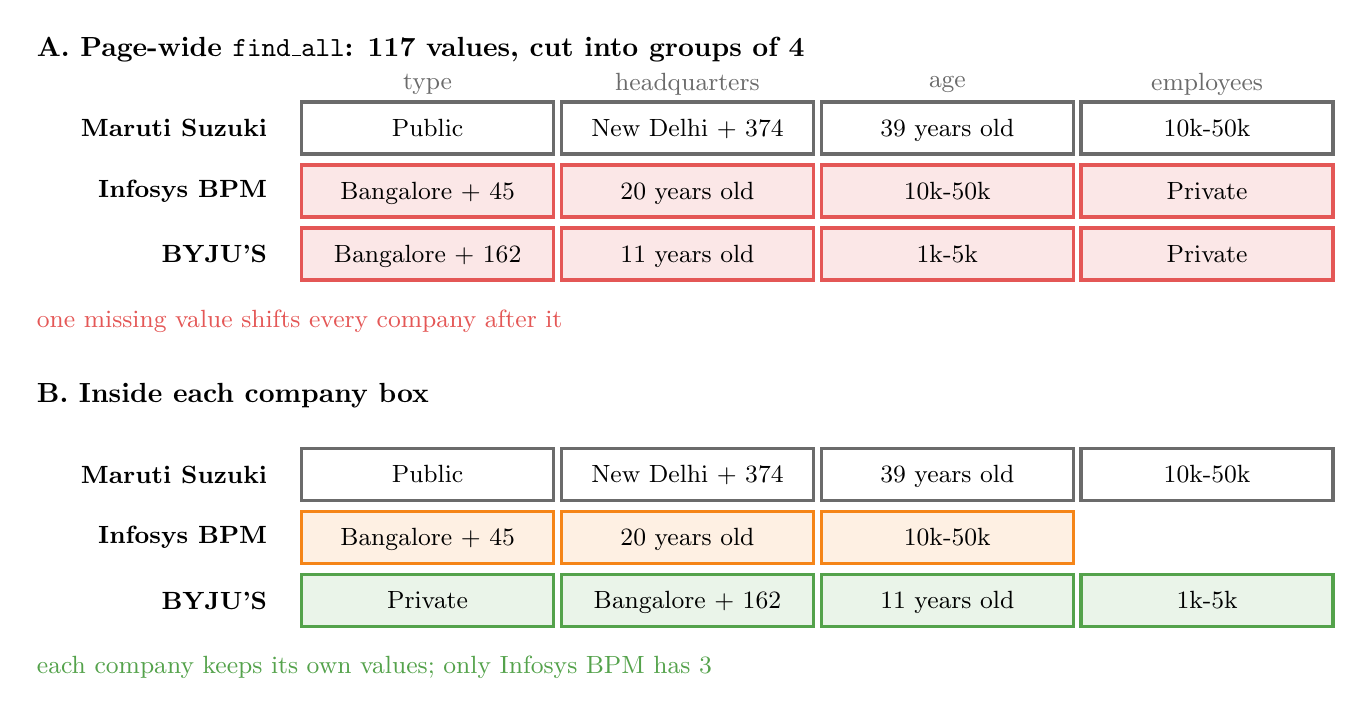
\begin{tikzpicture}[
    cell/.style={draw=cgrey, minimum width=3.2cm, minimum height=0.66cm, font=\small, text height=1.8ex, text depth=0.4ex},
    bad/.style={cell, draw=cred, fill=cred!14},
    nm/.style={font=\small\bfseries, anchor=east},
    hd/.style={font=\bfseries, anchor=west}]
  % ---- top: one long page-wide list, cut into groups of 4 ----
  \node[hd] at (-3.4,1.0) {A.\ Page-wide \texttt{find\_all}: 117 values, cut into groups of 4};
  \node[nm] at (-0.2,0) {Maruti Suzuki};
  \foreach \t [count=\i from 0] in {Public, New Delhi + 374, 39 years old, 10k-50k}
    \node[cell] at (1.7+\i*3.3,0) {\t};
  \node[nm] at (-0.2,-0.8) {Infosys BPM};
  \foreach \t [count=\i from 0] in {Bangalore + 45, 20 years old, 10k-50k}
    \node[bad] at (1.7+\i*3.3,-0.8) {\t};
  \node[bad] at (11.6,-0.8) {Private};
  \node[nm] at (-0.2,-1.6) {BYJU'S};
  \foreach \t [count=\i from 0] in {Bangalore + 162, 11 years old, 1k-5k, Private}
    \node[bad] at (1.7+\i*3.3,-1.6) {\t};
  \node[note, text=cred, anchor=west] at (-3.4,-2.45) {one missing value shifts every company after it};
  % ---- bottom: one container at a time ----
  \begin{scope}[shift={(0,-4.4)}]
    \node[hd] at (-3.4,1.0) {B.\ Inside each company box};
    \node[nm] at (-0.2,0) {Maruti Suzuki};
    \foreach \t [count=\i from 0] in {Public, New Delhi + 374, 39 years old, 10k-50k}
      \node[cell] at (1.7+\i*3.3,0) {\t};
    \node[nm] at (-0.2,-0.8) {Infosys BPM};
    \foreach \t [count=\i from 0] in {Bangalore + 45, 20 years old, 10k-50k}
      \node[cell, draw=corange, fill=corange!12] at (1.7+\i*3.3,-0.8) {\t};
    \node[nm] at (-0.2,-1.6) {BYJU'S};
    \foreach \t [count=\i from 0] in {Private, Bangalore + 162, 11 years old, 1k-5k}
      \node[cell, draw=cgreen, fill=cgreen!12] at (1.7+\i*3.3,-1.6) {\t};
    \node[note, text=cgreen, anchor=west] at (-3.4,-2.45) {each company keeps its own values; only Infosys BPM has 3};
  \end{scope}
  \foreach \t [count=\i from 0] in {type, headquarters, age, employees}
    \node[font=\small, text=cgrey] at (1.7+\i*3.3,0.55) {\t};
\end{tikzpicture}
\end{document}
